%% Bemærk:
%%          Resten af rapporten følger en stil hvor indledninger skrives
%%          med \sffamlily-typen. Denne stil bør også følges her.
%%
{\sffamily
I dette afsnit vil vi afprøve den generelde region detektor, det vil
sige hvad der egentlig bliver fundet inden, vores to metoder sortere
regionerne fra. selve metodes fremgangsmåde er beskravet i sektion
\ref{Sammensetning_af_metoder}, hvor det sideste skrid nå billedet
bliver floodfilldet, derfor vil vi forklare afprøvningen af metode ud
fra billeder som er kommer til dette skridt, hvor tærskelværdierne er
sat til de fundene tærskelværdier. Den første del vil omhandle test på
opbygget billeder og den anden del vil omhandle test på udvalgte
billeder fra vores billedet database.
}

\subsection{Afprøvning på test billeder}
I dette sektion tester vi på billeder som er konstrueret, men en hvid
baggrund og sorte regioner, det snit vi tester på er indtegnet samt
marginen. 

I billedet \ref{GRD_test1} er der 5 regioner, hvor 3 af dem bliver
fundet da de ligger i snittet, de 2 regioner som ikke er fundet er
stadig sorte, som man kan se bliver både den er krydser snittet og den
der tangere snittet taget med. 

\begin{figure}[!h]
    \centering
		\subfloat[4 figure og en bagrun, hvor 2 af figurene og bagrunden er fundet]{
        	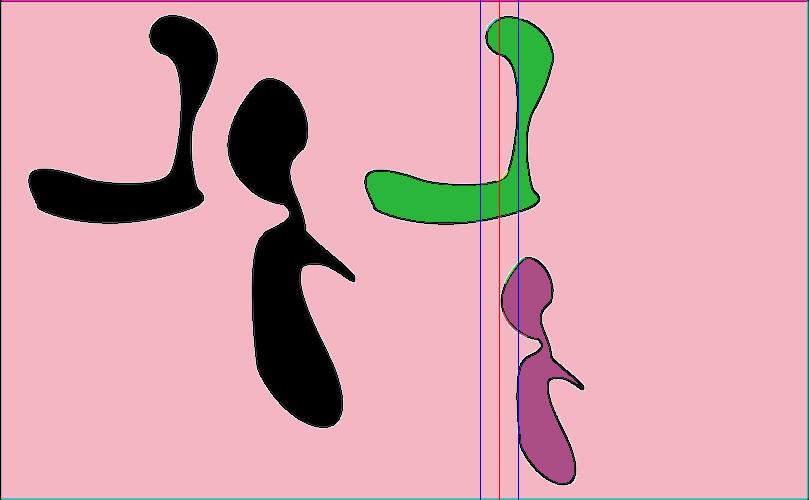
\includegraphics[angle=0,width=0.7\textwidth]{afsnit/afprovning/billeder/region_selector/blob_region_section.png}
        	\label{GRD_test1}}\hspace{1em}
    	\subfloat[Orginal]{
	       	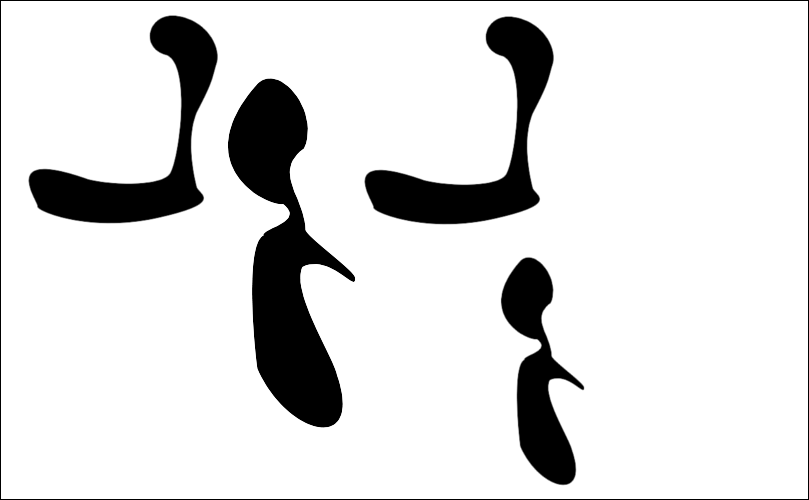
\includegraphics[angle=0,width=0.7\textwidth]{afsnit/afprovning/billeder/region_selector/blob_section.png}
	       	\label{GRD_test1_original}}\hspace{1em}
        \caption[]{}
     \label{GRD_test1_sammen}
\end{figure}

I billedet \ref{GRD_test2} er der 3 regioner som
alle bliver fundet, baggrunden, den lille region som ligger inde for
margin, og den store region som kun har en lille del af dens masse inde
i snittet. 

\begin{figure}[!h]
    \centering
		\subfloat[En stor figur og en lille figur begge fundet]{
        	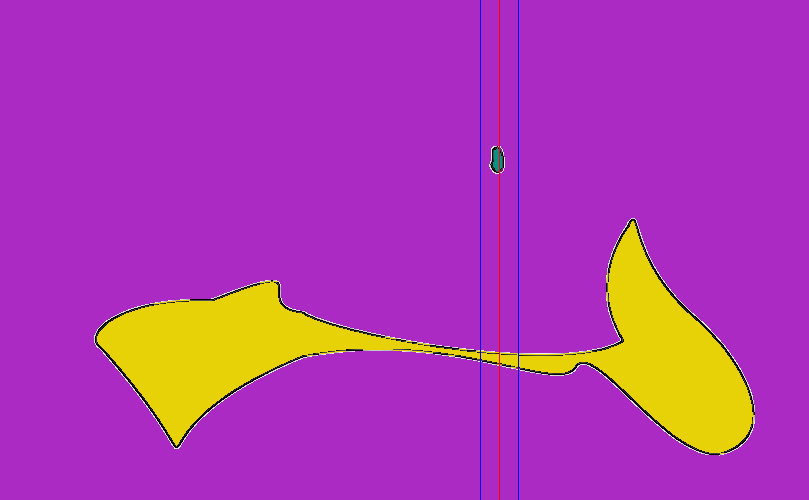
\includegraphics[angle=0,width=0.7\textwidth]{afsnit/afprovning/billeder/region_selector/blob2_region_section.png}
        	\label{GRD_test2}}\hspace{1em}
    	\subfloat[Orginal]{
	       	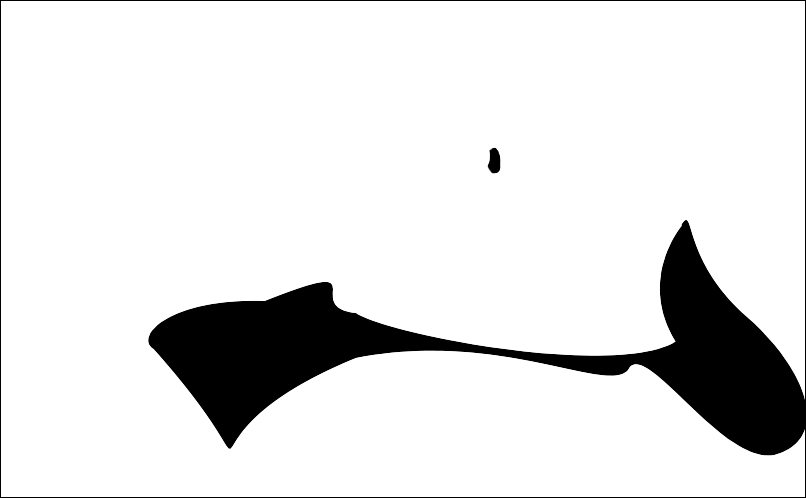
\includegraphics[angle=0,width=0.7\textwidth]{afsnit/afprovning/billeder/region_selector/lille_tvers.png}
	       	\label{GRD_test2_original}}\hspace{1em}
        \caption[]{}
     \label{GRD_test2_sammen}
\end{figure}

I billedet \ref{GRD_test3} er der en hoisont som ligger oven på
snittet, begge sider af hoisont linien bliver tegnet med.

\begin{figure}[!h]
    \centering
		\subfloat[En stor figur og en lille figur begge fundet]{
        	
\includegraphics[angle=0,width=0.7\textwidth]{afsnit/afprovning/billeder/region_selector/hoisont_region_section.png}
        	\label{GRD_test3}}\hspace{1em}
    	\subfloat[Orginal]{
	       	
\includegraphics[angle=0,width=0.7\textwidth]{afsnit/afprovning/billeder/region_selector/hoisont.png}
	       	\label{GRD_test3_original}}\hspace{1em}
        \caption[]{}
     \label{GRD_test3_sammen}
\end{figure}

I de 3 figur \ref{GRD_test1_sammen}, \ref{GRD_test1_sammen} og
\ref{GRD_test1_sammen} er de 3 test billeder afbilledet, de opføre sig
efter de standarter som vi frem satte i afsnit \ref{}XX(hvilken
reference?) og virker efter vores forventniger.

\subsection{Afprøvning på malerier}
Vi vil afprøve region detektor på 6 udvalte billeder, som vær viser
styrker og svagheder ved region detektoren

\begin{figure}[!h]
    \centering
		\subfloat[Maleri med Kraftige farver og få detaljer]{
        	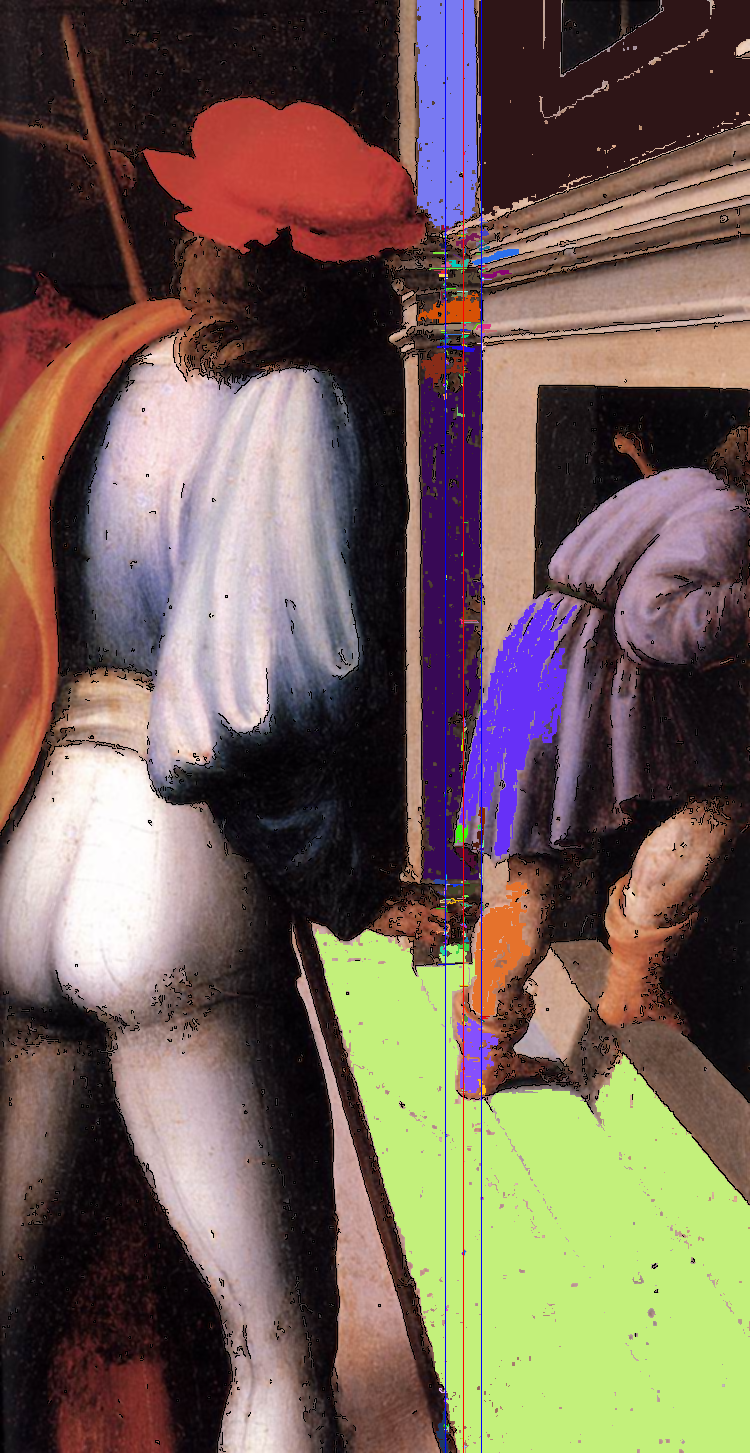
\includegraphics[angle=270,width=1.0\textwidth]{afsnit/afprovning/billeder/thressholds/krafitige_farver/svage_detalier/floodfill/4-4.png}
        	\label{GRD_virker1}}\hspace{1em}
		\subfloat[Medium farver og medium detaljer]{
        	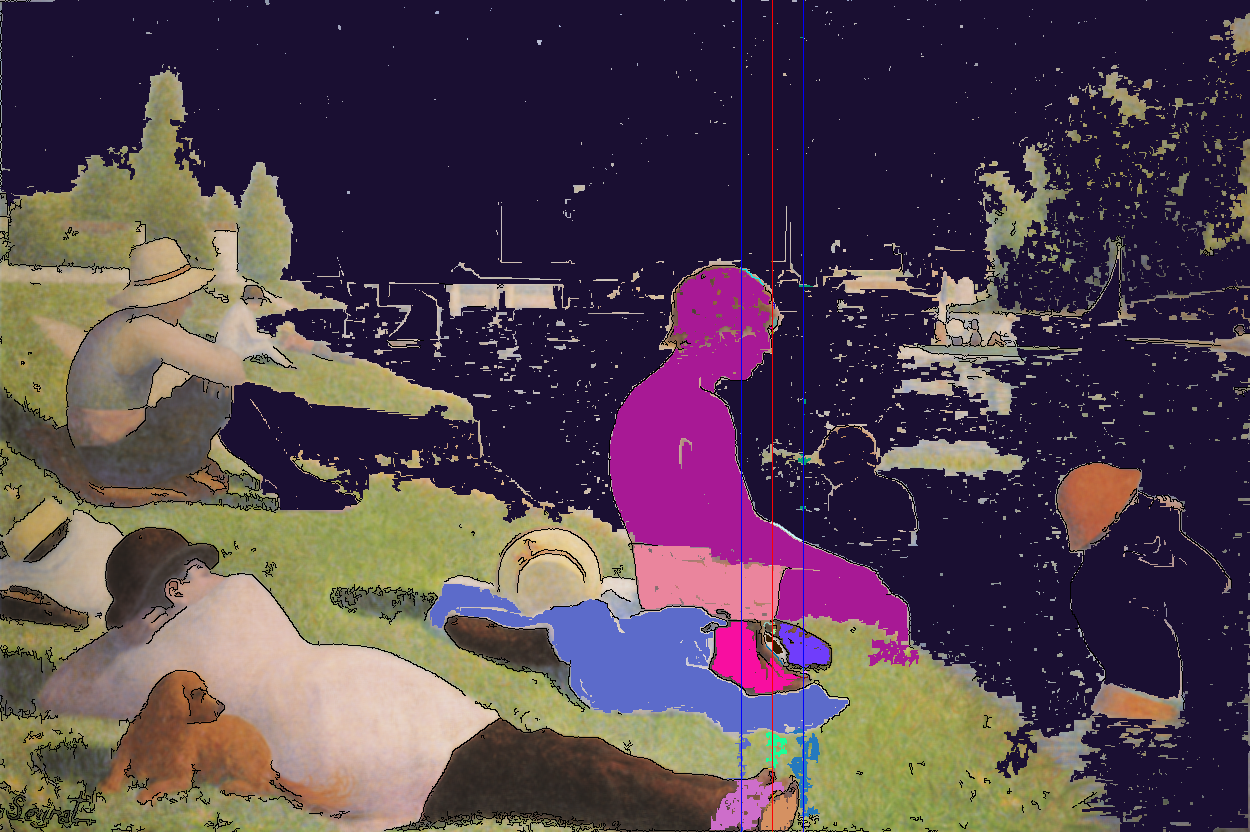
\includegraphics[angle=0,width=1.0\textwidth]{afsnit/afprovning/billeder/4-4.png}
        	\label{GRD_virker2}}\hspace{1em}
        \caption[]{2 malerier hvor regions detektoren virker efter vores ønsker}
     \label{generelde_region_detektor_virker}
\end{figure}

I figuren \ref{generelde_region_detektor_virker} er der 2 malerier, hvor
vores region detektor virker rigtige godt. 

Det første maleri \ref{GRD_virker1} finder region detektoren 7 store
regioner og en masse små, metoden finder forskel på de forskellige
paneler i kaminen og vært tøj stykke på personen i maleriet er blevet
vær deres region, de små regioner er samlet ved et skift fra et panel
til et andet og forstyrrer ikke de store region ved at gå i gennem dem,
man kunne måske have ønsket at den fylde lidt mere af han karpe ud, men
eller et meget godt eksempel på hvordan den generelde region detektor
finde lige det vi vil have den til at finde. 

I maleriet \ref{GRD_virker2} finder vi mange af de samme
godt ting, drengen i miden af maleriet er helt udfyldt, en sko og et
håndklæde er også fundet, det er dog vigtigt at ligge mærke til at de
andre personer i vandet, fylder i et med baggrunden, som normalt vil
være en dårlig ting, men som ikke gør noget her da, metoden kun ser
efter regioner i snittet, repræsenteret af den røde linie.
 
\begin{figure}[!h]
    \centering
		\subfloat[Kraftige farver og mange detaljer]{
       	 	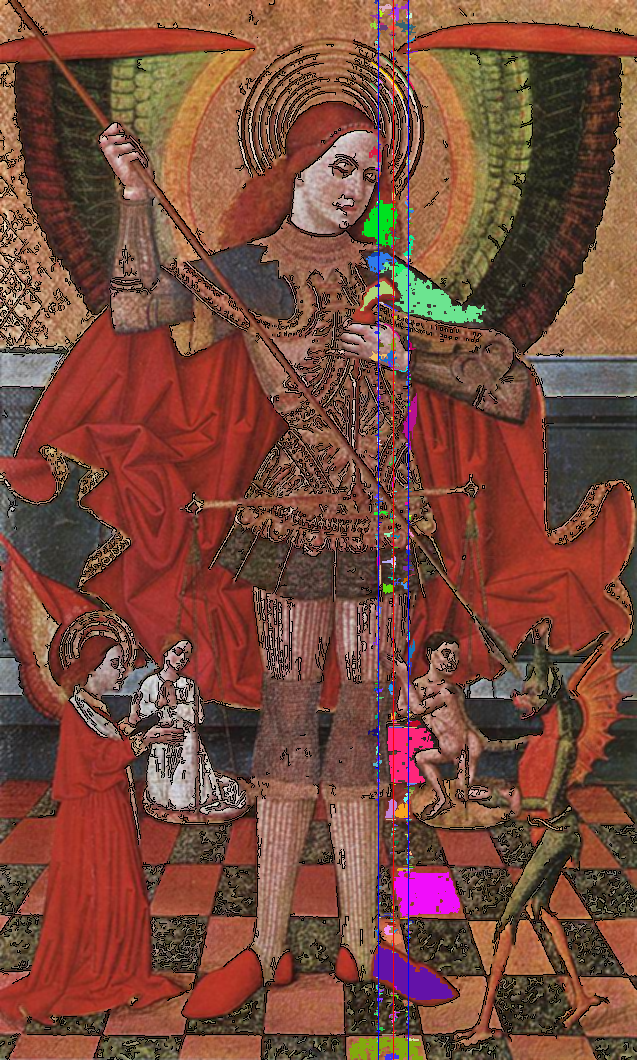
\includegraphics[angle=270,width=0.90\textwidth]{afsnit/afprovning/billeder/thressholds/krafitige_farver/krafite_detalier/floodfill/4-4.png}
		    \label{GRD_virker_nesten1}}\hspace{1em}
    \subfloat[Medium farver og medium detaljer]{
        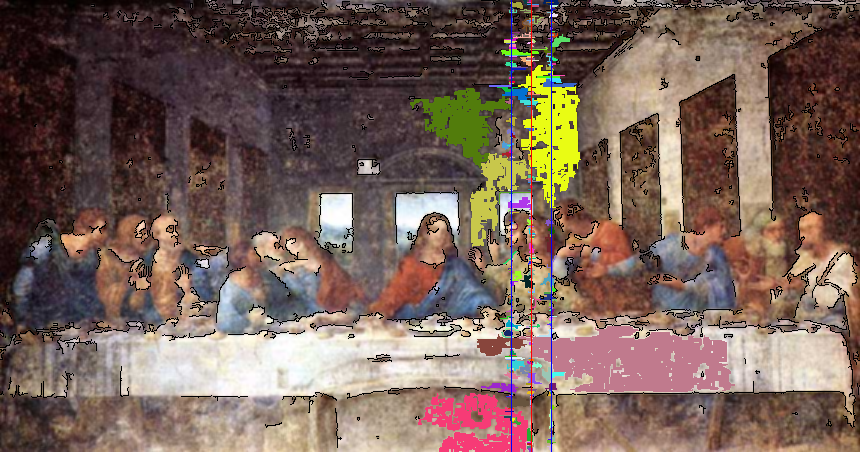
\includegraphics[angle=0,width=0.95\textwidth]{afsnit/afprovning/billeder/thressholds/medium_farver/medium_detalier/floodfill/4-4.png}
        \label{GRD_virker_nesten2}}\\
     \label{generelde_region_detektor_virker_nesten}
     \caption[]{2 malerier hvor regions detektoren ikke helt virker efter vores ønsker men stadig har noget vi kan bruge}
\end{figure}

I figuren \ref{generelde_region_detektor_virker_nesten} og er der 2
malerier, hvor vores region detektor ikke virker efter vores ønsker med
stadig har noget vi kan bruge. 

I maleriet \ref{GRD_virker_nesten1}
bliver der mest fundet små region dog bliver en sko, en skulder og en
flise fundet, hvor vi gerne vil have at personens karpe og arm også blev
fundet, dette skyldes primert at tærskelværdierne for dette billedet er
sat for lavt. 

Det andet maleri \ref{GRD_virker_nesten2} har nogle af de
samme problematiker, region detektoren finder mest en masse små stykker
af noget som burde hænge sammen. Det vil også kunne løses ved nogle
andre tærskelværdier, men som man også kan se på maleriet er væge og
loftet som egentlige er ret ensfarvet stadig svære for vores region
detektor at fange, det tyder på at en støre sløring godt kunne være
problemløseren få at algoritmen virker på dette maleri. 

Grunden til at lige de her 2 bilder er interessante er at ved ændring på
tærskelværdier og sløring kunne vores region detektor virker godt XX(her
skal der billeder hvor det virker), 

\begin{figure}[!h]
    \centering
    \subfloat[Kraftige farver og medium detaljer]{
        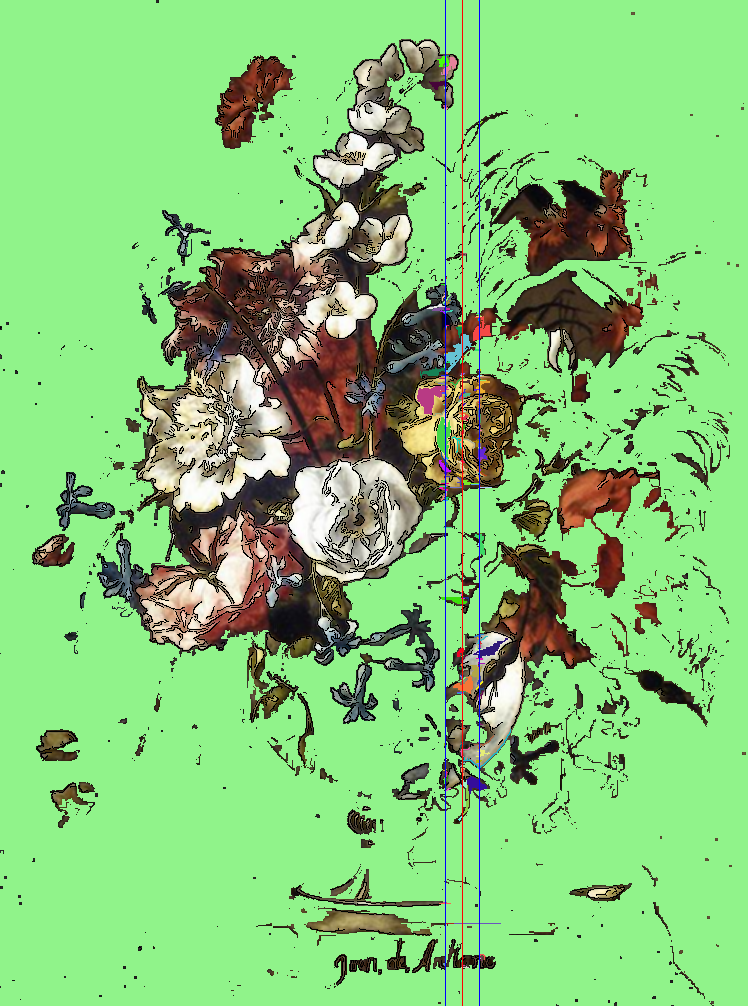
\includegraphics[angle=0,width=0.46\textwidth]{afsnit/afprovning/billeder/thressholds/krafitige_farver/medium_detalier/floodfill/4-4.png}
        \label{GRD_virker_ikke1}}
     \subfloat[Original]{
        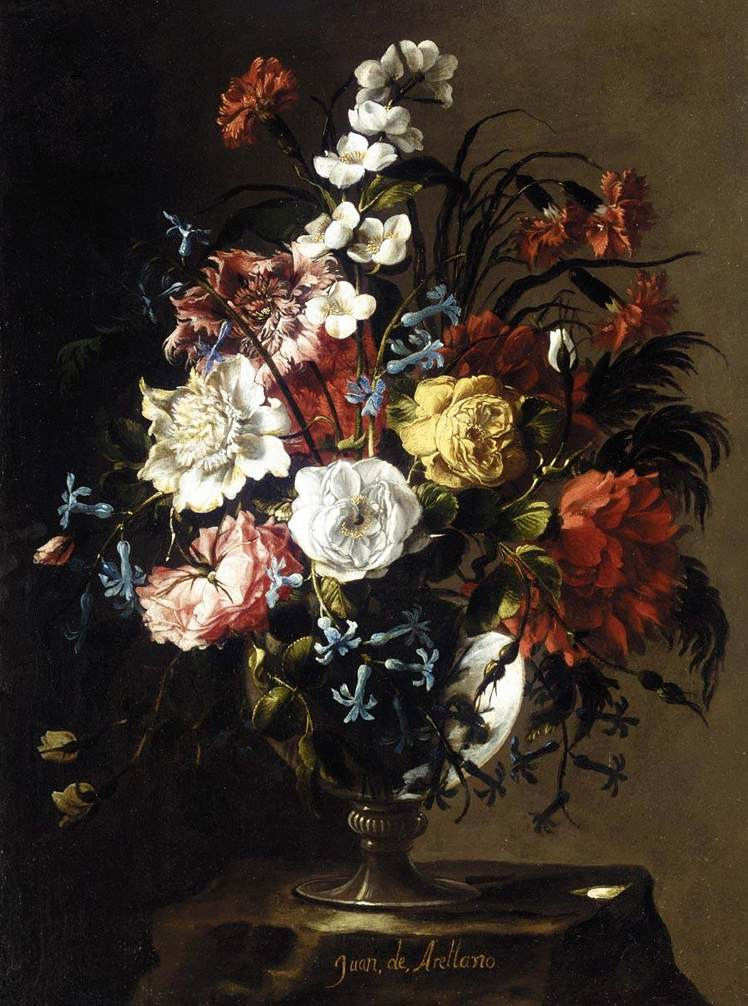
\includegraphics[angle=0,width=0.46\textwidth]{afsnit/afprovning/billeder/thressholds/krafitige_farver/medium_detalier/mDetalier}
        \label{GRD_virker_ikke1_orginal}}
     \label{generelde_region_detektor_virker_ikke}
     \caption{}
\end{figure}

\begin{figure}[!h]
    \centering
    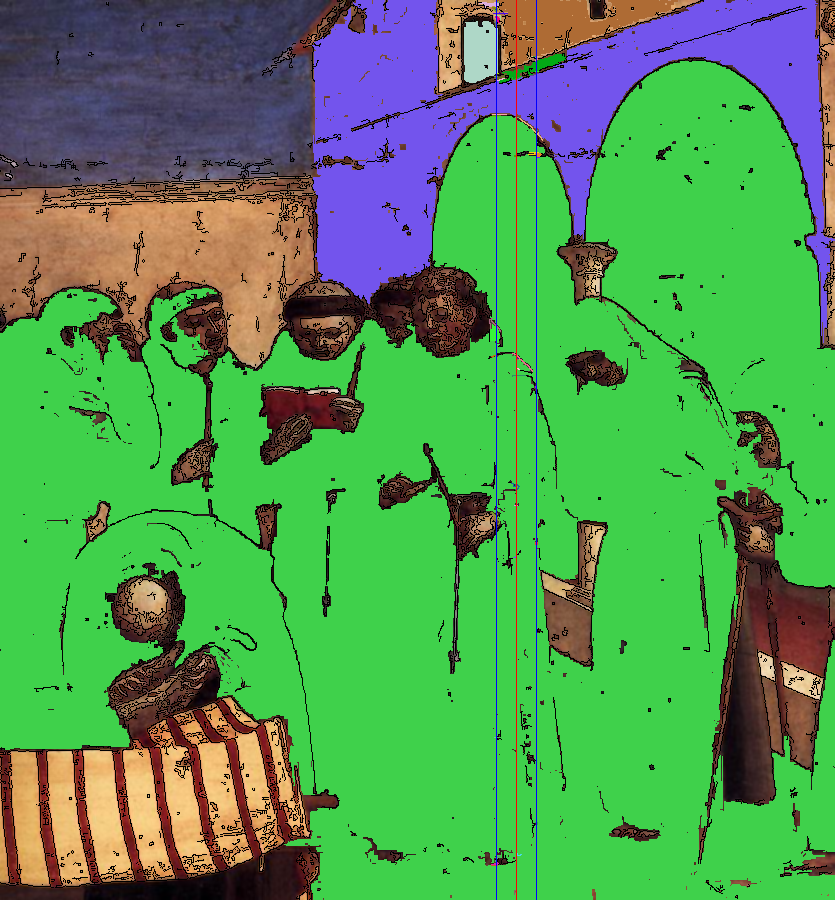
\includegraphics[angle=0,width=0.65\textwidth]{afsnit/afprovning/billeder/thressholds/svage_farver/svage_detalier/floodfill/4-4.png}
    \caption{Svage farver og få detaljer}
    \label{GRD_virker_ikke2}
\end{figure}

I figur \ref{generelde_region_detektor_virker_ikke} og
\ref{generelde_region_detektor_virker_ikke2} er der 2 malerier hvor
vores region detektor ikke virker særlige godt. 

I maleri \ref{GRD_virker_ikke1} er noget af buketten og baggrunden gået
i et. På samme tid er resten af blomsterne i snittet ikke fyldt ud, og
selv med en ændring i tærskelværdierne vil det ikke hjælpe, da en øgning
af tærskelværdierne vil resultere i at flere af blomsterne gå i et med
baggrunden, og en sænkning, vil resultere i at ingen af blomsterne vil
blive detektet. 

Maleriet \ref{GRD_virker_ikke2} har en anden problemstiling som vi ikke
kan komme uden om, farverne er så mørke og svage at en ændring i
tærskelværdien i floodfill på bare 1 vil få regiondetektoren til at gå
fra at finde ingen regioner til at finde en stor, som på billedet, dette
kan også skyldes at kantdetektionen tilføje en mørk kan rundt om
regionerne, men da maleriet er mørkt i forvejen hjælper kandetektionen
ikke. XX(jeg kan ikke helt prolamere dette unden at have nogle bileder
at bagge det op)

